\chapter{ \MakeUppercase{MUOGRAFÍA}}
\label{ch:c_rays}

El estudio de grandes estructuras mediante muografía se basa en el principio de la radiografía, es decir, la radiación a la que se expone un objeto es absorbida parcialmente dependiendo de su densidad. La muografía utiliza como fuente de radiación los muones atmosféricos creados por la interacción de los rayos cósmicos con los átomos que componen la atmósfera terrestre. Los muones interactúan con los átomos que conforman el objeto escaneado, creando procesos de pérdida de energía y dispersión múltiple \footcite{procureur2018muon}.

Todas las aplicaciones de la muografía se basan en la atenuación del flujo de muones al atravesar un objetivo, aprovechando el flujo natural de muones producido por las interacciones de los rayos cósmicos en la atmósfera\footcite{bonechi2020atmospheric}.

La primera aparición práctica de muografía se remonta a la década de 1950, cuando George estudió la viabilidad de emplear un telescopio Geiger para inferir el espesor del hielo sobre un túnel en una mina australiana \footcite{george1955cosmic}.

Hoy en día, la vulcanología es el área que más implementa la muografía, ya que esta proporciona información del comportamiento dinámico de dichas formaciones geológicas de manera no invasiva y con una resolución espacial de decenas de metros\footcite{Tanaka2005}.
  
 
\section{Muones atmosféricos}
Cuando la CR llega a la Tierra colisiona con los núcleos atómicos en la atmósfera. Produciendo nuevas partículas que posteriormente chocan con otros núcleos, creando una nueva generación de partículas que continúan el proceso. La cascada de partículas resultante es llamada lluvia aérea extensa (EAS por sus siglas en inglés). Las EAS pueden llegar al nivel del suelo extendiéndose sobre grandes áreas ($\approx$ km$^{2}$).
 
 \begin{figure}[h]
    \begin{center}
        \caption[Componentes de la lluvia aérea extendida(EAS)]{Componentes de la lluvia aérea extendida (EAS):
        hadrónica (verde), electromagnética (roja) y muónica (azul\textbf{}).}
        \includegraphics[width=0.78
        \textwidth]{Figures/imagenes/EAS_Components}
        \caption*{\textbf{Fuente.} \cite{Haungs2011}. }
        \label{Components}
    \end{center}
\end{figure}
 
Las EAS están conformadas por tres componentes: la \textbf{electromagnética}, la \textbf{hadrónica} y la componente \textbf{muónica} como se muestra en la Fig.\ref{Components}. La interacción de la CR en la atmósfera produce cascadas de partículas más ligeras como los piones ( $\pi^{+},\pi^{0},\pi^{-})$ y kaones $(K^{+},K^{0},K^{-})$ los cuales se descomponen principalmente en muones \footcite{tanabashi2018review}. Los muones, en comparación con otras partículas inestables, pueden desplazarse grandes distancias en la atmósfera sin decaer. Los muones conforman más de la mitad de la radiación cósmica a nivel del mar, siendo el resto principalmente electrones, positrones y fotones provenientes de las EAS. 


\section{Fuentes de ruido en muografía}
La muografía tiene principalmente tres fuentes de ruido: los muones de baja energía dispersados por la superficie de la estructura escaneada, las partículas que ingresan por la parte posterior del detector y la componente electromagnética de las EAS. Si el ruido de fondo es dominante en la observación, la densidad estimada será menor que la densidad real. 


\subsection{Dispersión de muones de baja energía}

El flujo de muones a grandes ángulos cenitales es bajo y los muones dispersados en la estructura escaneada pueden volverse fácilmente dominantes. En este caso, la dirección del muón incidente varía debido a la dispersión múltiple de Coulomb generada por su interacción con la estructura escaneada \footcite{bonechi2020atmospheric}. La dispersión angular  causa un desenfoque de la imagen final de densidad, afectando su resolución espacial con la consiguiente pérdida de detalles.

\begin{figure}[H]
    \begin{center}
        \caption[Dispersión de los muones incidentes de baja energía sobre la superficie]{Dispersión de los muones incidentes de baja energía sobre la superficie. El ángulo de incidencia del muón $\theta_{ini}$ varía debido a su interacción con el material que compone la estructura resultando en un ángulo dispersado $\theta_{fin}$.}
        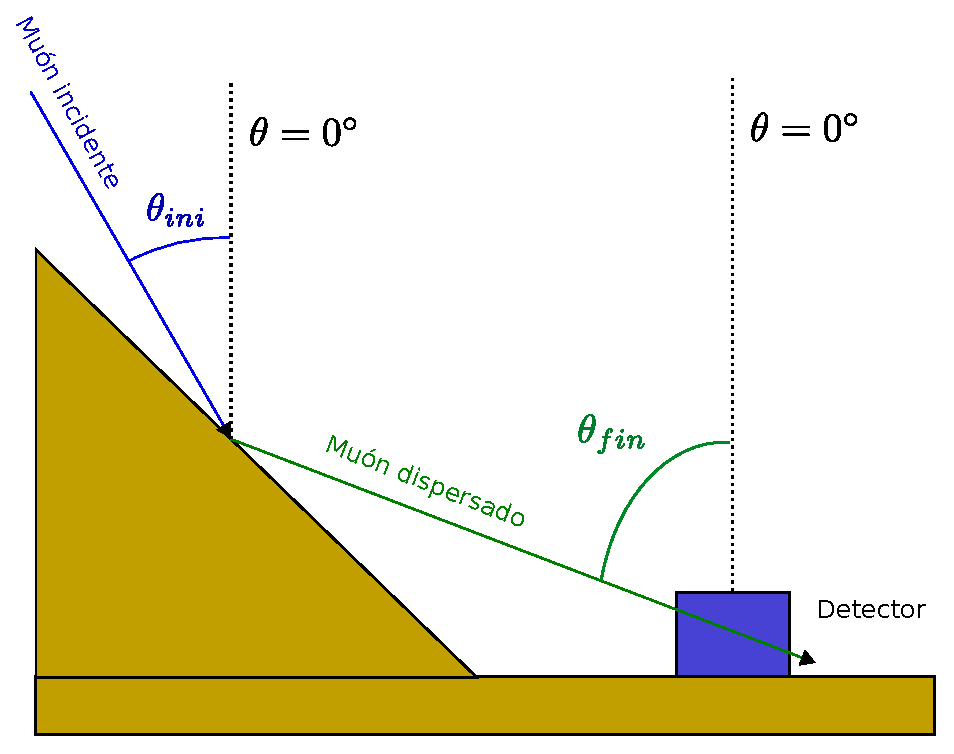
\includegraphics[width=0.6\textwidth]{Figures/imagenes/Muon_scattering.eps}
        \caption*{\textbf{Fuente.} \cite{jesusP}. }
        \label{Scattering}
    \end{center}
\end{figure}


\subsection{Partículas de trayectoria inversa}

Otra fuente de contaminación en la muografía son las partículas que impactan en el detector desde la parte posterior\footcite{Nishiyama2014}, creando trayectorias similares a los mounes provenientes desde la estructura escaneada. Ver Fig. \ref{Albedo}.

\begin{figure}[H]
    \begin{center}
        \caption[Evento falso debido a un muón que incide por la parte posterior del detector]{Evento falso debido a un muón que incide por la parte posterior del detector.}
        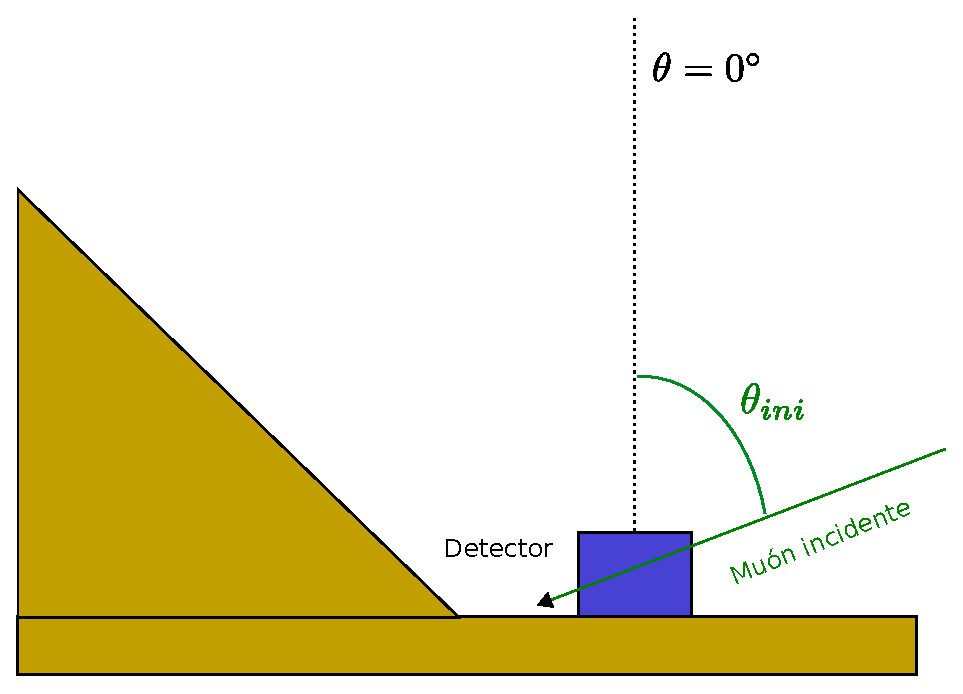
\includegraphics[width=0.6\textwidth]{Figures/imagenes/Albedo.eps}
        \caption*{\textbf{Fuente.} \cite{jesusP}. }
        \label{Albedo}
    \end{center}
\end{figure}

 
Los flujos traseros se detectan cuando la parte posterior del telescopio está expuesta a un amplio volumen de atmósfera ubicado por debajo del nivel de medición, como se observa en la Fig. \ref{topograf}. El análisis de datos discutido por Jourde et. al. \footcite{jourde2013experimental}, demuestra la existencia de un flujo de mounes traseros cuyas trayectorias podrían confundirse con la de los mounes descendentes que cruzan el volcán.


\begin{figure}[H]
    \begin{center}
        \caption{Resultado de la tomografía de alta definición en el Monte La Soufriere, sin corrección de flujo ascendente (Arriba) y con corrección de flujo ascendente (Abajo). Densidad de roca en $g.cm^{-3}$ }
        \includegraphics[width=0.65\textwidth]{Figures/imagenes/tomografia.png}
        \caption*{\textbf{Fuente.} \cite{jourde2013effects}. }
        \label{topograf}
    \end{center}
\end{figure}


Se reporta que los muones posteriores superan a los frontales dos a uno, respectivamente \footcite{jourde2013experimental}. El ruido inverso disminuye al aumentar el ángulo de elevación del telescopio. 

\subsection{Componente electromagnética}
 
Otra fuente de contaminación en la muografía ocurre a las partículas secundarias generadas por EAS entre la estructura y el detector. El flujo de PS a nivel del suelo está conformado principalmente por $\mu^{\pm}, e^{\pm}$ y $\gamma$ \ref{EAS}.

\begin{figure}[H]
    \begin{center}
        \caption[Detección de un evento falso debido a la incidencia de un $e^-$ generado en una EAS entre el objeto escaneado y el detector]{Detección de un evento falso debido a la incidencia de un $e^-$ generado en una EAS entre el objeto escaneado y el detector.}
        \includegraphics[width=0.65\textwidth]{Figures/imagenes/EAS.eps}
        \caption*{\textbf{Fuente.} \cite{jesusP}. }
        \label{EAS}
    \end{center}
\end{figure}

Las partículas secundarias generan falsa información de dos maneras:

\begin{itemize}
    \item Mediante la coincidencia accidental de dos o más partículas incidentes en el detector lo cual imita una trayectoria generada por un muón \footcite{KUSAGAYA2015}.
    
    \item Un electrón/positrón con energía suficiente para atravesar todo el detector.
\end{itemize}
    
Teniendo en cuenta que la muografía calcula la distribución densidad interna de la estructura dependiendo del flujo diferencial de los mounes que la atraviesan, un aumento en el flujo registrado debido a los eventos falsos repercute en la medición de la densidad de la estructura. \footcite{Nishiyama2014}.  

\subsection{Incidencia múltiple de partículas}
El ruido combinacional es causado por varias partículas individuales que golpean los paneles sensibles, confundiendo al detector como si fuera un evento generado por una única partícula (Ver Fig. \ref{Mult}). Estos eventos tienen la singularidad que las partículas están correlacionadas temporalmente, ya que son producidas por la misma EAS \footcite{jesusP}. 


\begin{figure}[H]
    \begin{center}
        \caption{Electrones  generados por una EAS, causando un evento de múltiple partícula que imita un evento causado por una partícula única.}
        \includegraphics[width=0.65\textwidth]{Figures/imagenes/50.png}
        \caption*{\textbf{Fuente.} \cite{jesusP}. }
        \label{Mult}
    \end{center}
\end{figure}

El retardo en promedio de los muones para una distancia al centro de la EAS menor a 1km es $<$ a 100 ns, se puede jugar con esos datos para combatir con el ruido combinacional. También se puede reducir aumentando el número de planos sensibles.

% Eliminación de ruido
\section{Eliminación de ruido en muografía}
 Debido a los altos niveles de ruido en la muografía generados por las diferentes fuentes antes mencionadas, la eliminación de ruido en muografía se convierte en un campo para indagar. Se han creado distintos métodos para la disminución del ruido en la muografía, algunos que sobresalen son la adicción de capas del material absorbente, el aumento de capas sensibles y la medición del ToF. Estos se pueden clasificar en métodos activos y pasivos.  

\begin{figure}[H]
    \begin{center}
        \caption{(Arriba a la izquierda) Muón falso. Causado por un hadrón de EAS (Arriba a la derecha) Ruido combinatorio. (Abajo a la izquierda) Muón de bajo momentum. (Abajo a la derecha) Muón de de trayectoria inversa }
        \includegraphics[width=0.86\textwidth]{Figures/imagenes/noise.jpg}
        \caption*{\textbf{Fuente.} \cite{bonechi2020atmospheric}. }
        \label{ruido}
    \end{center}
\end{figure}


\subsection{Métodos activos}

Estos métodos buscan la eliminación de fuentes de ruido mediante el análisis de los datos entregados, para encontrar un patrón que muestre el comportamiento del los eventos falsos.

L. Oláh et. al. \footcite{olah2018high} implementaron siete detectores tipo cámara proporcional de múlti-hilo (MWPC), con un tamaño de ($ 80 \times 80$ cm$^{2}$), con cinco láminas de protección contra la radiación construidas de plomo, cada placa está oculta dentro de otra caja de acero inoxidable para protegerla mecánicamente y evitar la exposición a la toxicidad del plomo. La Fig. \ref{multi} muestra el detector desde una vista lateral.

 Debido a la buena resolución espacial, la dispersión de partículas de baja energía en las placas de plomo se puede medir a lo largo de la trayectoria y, por lo tanto, estas partículas de fondo $< 2$ GeVc$^{-1}$ se pueden eliminar de los datos registrados. 
 
  
  \begin{figure}[H]
    \begin{center}
        \caption{El sistema de observación muográfica basado en MWPC (mMOS). La vista esquemática de mMOS que consta de siete cámaras proporcionales multi-hilo y cinco placas de blindaje de plomo con un grosor de 2 cm cada una }
        \includegraphics[width=0.6\textwidth]{Figures/imagenes/multi.png}
        \caption*{\textbf{Fuente.} \cite{Olh2018}. }
        \label{multi}
    \end{center}
\end{figure}
Dentro de los métodos activos se encuentra la medición del tiempo de vuelo (ToF). EL ToF es el tiempo que tarda una partícula en recorrer una distancia determinada. Con esta  estimación se pueden calcular otras variables como velocidad, momento, dirección e identidad. 
El momento \textit{p} se relaciona con el ToF mediante:

\begin{equation}
    p= \frac{m_ocd}{\sqrt{c^2t^2-d^2}}
\label{MOM}
\end{equation}

Donde $m_o$ es la masa de la partícula cargada en reposo, c es la velocidad de la luz, d es la distancia recorrida y t es el tiempo de vuelo. 

% Parte del párrafo que cita la imagen.

La Fig. \ref{tof} muestra el ToF en función del ángulo cenital, las elipses sólidas identifican a los muones que se propagan hacia abajo (componente principal del flujo), las elipses discontinuas muestran la existencia de muones con propagación hacia arriba identificadas por el detector. Los resultados para la medición presentada en la figura muestran que la contaminación asciende al 70$\%$ del flujo total, y disminuye al 30$\%$ en ángulos de -10° y en cero por encima de -20°. Estos resultado permiten corregir las imágenes obtenidas por el detector \footcite{Marteau2014}.


 \begin{figure}[h]
    \begin{center}
        \caption{Distribución del ToF en función del ángulo cenital para los datos registrados en el volcán La Soufriere. El horizonte está representado por la línea discontinua. Las elipses sólidas azul y roja muestran respectivamente los eventos hacia atrás ($\alpha_{B}  < 0 $  y $\bigtriangleup t < 0$ ) y hacia adelante ($\alpha_{F} < 0$ y $\bigtriangleup t > 0$) correspondientes a los flujos descendentes. Las elipses discontinuas muestran eventos correspondientes a muones ascendentes desde adelante (elipse roja, $\alpha_{B} < 0$ y $\bigtriangleup t > 0$) y hacia atrás (elipse azul, $\alpha_{F} < 0$ y $\bigtriangleup t <0$) }
        \includegraphics[width=0.57\textwidth]{Figures/imagenes/ToF.png}
        \caption*{\textbf{Fuente.} \cite{jourde2013effects}. }
        \label{tof}
    \end{center}
\end{figure} 
 
\subsection{Métodos pasivos}
Este método consiste en adicionar capas de material absorbente entre los paneles del hodoscopio. Lo que se busca es que la partícula que atraviesa el detector pierda toda su energía en el material absorbente.
La primera implementación de esta técnica fue hecha por Nagamine et. al. \footcite{Nishiyama2014}, donde introducen dos placas absorbentes de hierro (40 g/cm$^{2}$) dentro del sistema de detección para filtra los muones de baja energía ($< 1 GeVc^{-1}$).

 

